\documentclass{article}
\usepackage{graphicx}
\usepackage[affil-it]{authblk}
\usepackage{url}
\usepackage{nth}
\usepackage{float}
\usepackage{multirow}

\begin{document}

\title{Developing a driver for a film scanner by means of USB sniffing and reverse engineering}
\author{Hugo Platzer \\ University of Salzburg}
\maketitle

\section{The USB standard}

\subsection{Motivation}

USB is an interface intended to connect various peripherals to PCs. These include:
Human interface devices like keyboards and mice; storage devices like card readers,
external hard disks, memory sticks and smartphones; multimedia devices like microphones, speakers,
cameras and scanners. Some highlights leading to its wide adoption:

\begin{itemize}
  \item Unified interface for all kinds of peripherals
  \item Plug and play: The user plugs in the device, the configuration (e.g. loading the appropriate drivers)
  is done automatically by the operating system
  \item Number of ports can be increased using hubs. Multiple hubs can be chained
        allowing for up to 127 devices on a single root port.
  \item High data rate of 480 Mbit / s (USB 2.0 high-speed mode). Also offers low-latency
        transfers for real-time audio/video applications
  \item Backwards compatibility: Older USB 1.1 devices can be used at 2.0 hosts.
        High-speed USB 2.0 devices can also be used on older
        machines supporting only USB 1.1 (albeit at lower speed).
\end{itemize}

\subsection{Electrical side}

\begin{figure}[!htbp]
  \caption{USB cable cross-section}
  \centering
  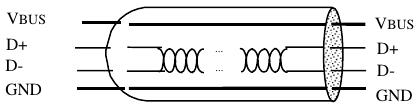
\includegraphics[width=0.5\textwidth]{images/usb_cable.jpg}
\end{figure}

A USB cable has four wires: One as ground, VBUS for a 5 V power supply and two for data transmission.
The power line allows it to draw up to 100 mA without any configuration. This is useful for simple
devices that are not using the data lanes, just the power, like USB lights. Also it allows for devices
not taking much power to be self-powered which eliminates the need for an extra power supply and connector.
Devices can ask the host for more power (up to 500 mA), those that need even more (like a lot of scanners) need
an external supply.

\subsection{Signaling}

\subsubsection{Low-level states}

USB is a serial bus which means there is only a single path for data transmission.
Differential signalling across the D- and D+ wires is used, which means the difference in voltage
across the two wires (rather than some absolute) determines the state. This is beneficial because
noise during transmission should affect both lines equally, not changing the difference.
Higher frequencies and thus data rates become possible.

\begin{table}[!htbp]
  \caption{USB speed modes}
  \centering
  \begin{tabular}{l | l | l}
    Mode & Speed & Bit time \\ \hline
    Low Speed & 1.5 Mbit / s & 667 ns \\
    Full Speed & 12 Mbit / s & 83 ns \\
    High Speed & 480 Mbit / s & 2 ns \\
  \end{tabular}
\end{table}

\begin{table}[!htbp]
  \caption{Low-level data line states (only applies to Full Speed)}
  \centering
  \begin{tabular}{l | l}
    Levels & State \\ \hline
    Differential '0' & D- high, D+ low \\
    Differential '1' & D- low, D+ high \\
    Single Ended Zero (SE0) & both low \\
    Single Ended One (SE1) & both high (illegal state, should never happen) \\
    Data 'J' state & Differential '1' \\
    Data 'K' state & Differential '0' \\
    Idle state & Data 'J' state \\
    Start of Packet (SOP) & Switch from idle to 'K' \\
    End of Packet (EOP) & SE0 for 2 bit times followed by 'J' for 1 bit time \\
    Disconnect & SE0 for $\geq$ 2 us \\
    Connect & Idle for 2.5 us \\
    Reset & SE0 for $\geq$ 2.5 us \\
  \end{tabular}
\end{table}

\pagebreak
Low Speed is used for devices where speed is not important (mice, keyboards).
It allows for cheaper cables and electronics. High Speed is only available
in USB 2.0. For reasons of simplicity, only full speed signaling will be covered
here.

SE0 is the state of the data lines if no device is connected. The host
recognizes a device being plugged in by the D+ line being "pulled up" to high.
It then most likely initiates a reset so the device is in a known state for
communication to begin. Similarly, a disconnect is sensed by a SE0 for some time.

It is important to note that {\bf all communication on the USB bus is initiated by the
host}. Devices on the bus can not directly talk to each other and can only talk
to the host as a direct response to a request made by it before.

\subsubsection{Bitstream encoding}

USB uses NRZI encoding for the transmitted data: A zero is represented by a change to
the opposite state while a one is represented by staying in the same state.

\begin{figure}[!htbp]
  \caption{NRZI bitstream encoding}
  \centering
  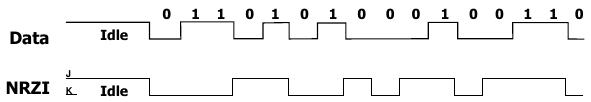
\includegraphics[width=0.5\textwidth]{images/nrzi_encoding.jpg}
\end{figure}

For keeping the receiver clock in sync with the data it is not ideal if the signal
stays at J or K for too long. To prevent this, a technique called "bit stuffing"
is used: Before doing NRZI encoding, a zero is inserted after every six consecutive ones
in the data. The receiver recognizes the stuffed bits during decoding and discards them.

\subsection {Packets}

Packets are the atomic unit of data transmission in USB. In between packet transmission,
the bus remains in an idle state. Every packet starts with a sync pattern to synchronize
the clocks between sender and receiver. Next are the actual data bits. The packet is
terminated by an EOP state. Fields in a packet are transmitted least-significant
bit first.

The first 8 bits of every packet contain the packet ID (PID) which identifies its type
and thus how the rest of the packet data should be interpreted. The PID is 4 bits long, they are transmitted a second time in reverse bit order to allow the receiver to quickly
discard a faulty packet. There are 17 different packet types (PRE and ERR have the same ID,
some are only relevant for High Speed):

\begin{table}[!htbp]
  \caption{USB packet types; notice how the least-significant two bits identify the packet category}
  \centering
  \begin{tabular}{l | l | l | p{5cm}}
    PID type & PID name & \begin{tabular}{@{}l} PID bits \\ ($<3:0>$) \end{tabular} & Description \\ \hline
    \multirow{4}*{Token} & OUT & 0001 & Address + endpoint number for host-to-device transaction \\
                         & IN & 1001 & Address + endpoint number for device-to-host transaction \\
                         & SOF & 0101 & Start-of-frame marker, frame number \\
                         & SETUP & 1101 & Special host-to-device transaction for device configuration \\ \hline
    \multirow{4}*{Data} & DATA0 & 0011 & Data packet \\
                         & DATA1 & 1011 & Data packet \\
                         & DATA2 & 0111 & Data packet (only High Speed) \\
                         & MDATA & 1111 & Data packet (only High Speed) \\ \hline
    \multirow{4}*{Handshake} & ACK & 0010 & Receiver accepts error-free data packet \\
                         & NAK & 1010 & Receiver cannot accept data or transmitter cannot send data \\
                         & STALL & 1110 & Endpoint halted or control pipe request not supported \\
                         & NYET & 0110 & Data packet (only High Speed) \\ \hline
    \multirow{4}*{Special} & PRE & 1100 & Preamble to enable downstream traffic to low-speed devices \\
                         & ERR & 1100 & Split Transaction error handshake \\
                         & SPLIT & 1000 & High speed Split Transaction token (only High Speed) \\
                         & PING & 0100 & High speed control flow probe (only High Speed) \\
                         & Reserved & 0000 & Reserved PID \\
  \end{tabular}
\end{table}

\subsubsection{Token packet}

\begin{figure}[H]
  \caption{Token packet composition}
  \centering
  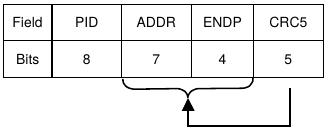
\includegraphics[width=0.5\textwidth]{images/token_packet.jpg}
\end{figure}

Token packets are used at the start of so-called transactions to specify the target
of the transaction on the bus, namely a certain device and endpoint. There are 127
possible devices on a bus (address 0 is reserved for a device that has not been configured yet).

Endpoints are logical entities on a device that are used as sources and sinks of data
in so-called pipes. A pipe is either in OUT (to device) or IN (to host) direction.
Endpoint 0 is a special bidirectional pipe that must be available on every device
right after the reset. It is used mainly for identifying and configuring the device.

\subsubsection{Data packet}

\begin{figure}[H]
  \caption{Data packet composition}
  \centering
  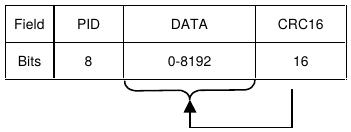
\includegraphics[width=0.5\textwidth]{images/data_packet.jpg}
\end{figure}

Used to transmit the actual data in a transaction.

\subsubsection{Handshake packet}

\begin{figure}[H]
  \caption{Handshake packet composition}
  \centering
  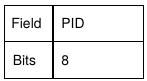
\includegraphics[width=0.21\textwidth]{images/handshake_packet.jpg}
\end{figure}

Used to report the status of a transaction.

\subsection{Transactions}

\subsection{Transfers}

\begin{figure}[H]
  \caption{Composition of a USB transfer}
  \centering
  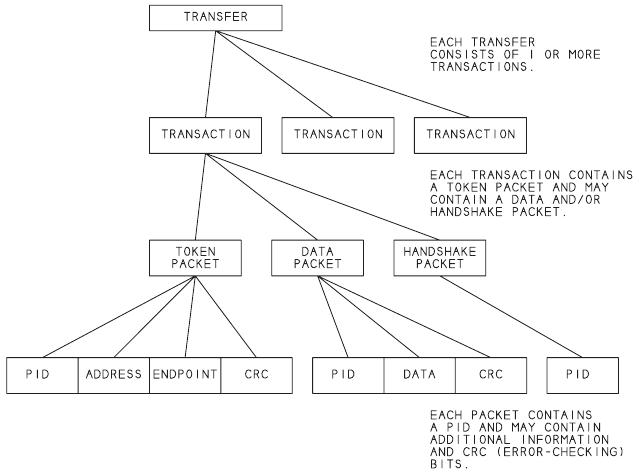
\includegraphics[width=\textwidth]{images/transfer_tree.jpg}
\end{figure}

\subsubsection {Control transfer}

\subsubsection {Interrupt transfer}

\subsubsection {Bulk transfer}

\subsubsection {Isochronous transfer}

\subsection{Enumeration, Configuration}

\begin{thebibliography}{}

\bibitem{usbstd}
Universal Serial Bus Specification, Revision 2.0. April 27, 2000. Available at \url{http://www.usb.org/developers/docs/usb20_docs/}

\bibitem{uc}
USB Complete: Everything You Need to Develop Custom USB Peripherals (\nth{3} edition).
Jan Axelson, Lakeview Research LLC 2012. ISBN: {\tt   978-1-931448-03-1}


\end{thebibliography}

\end{document}
